%!TEX root = Funktionalanalysis - Vorlesung.tex


\section{Trennungssätze für konvexe Menge}



\begin{motivation}
	todo, siehe Werner S.100/101 % todo motivation, siehe Werner S100/101
\end{motivation}


\begin{definition}
	Sei $X$ ein Vektorraum mit $A \subset X$. Definiere 
		\[ p_{A} \colon X \rightarrow [0, \infty], ~ p_{A}(x) \coloneqq \inf \{ \lambda > 0 : \frac{x}{\lambda} \in A \} \quad \text{(Minkowski-Funktional)} \]
	$A$ hei{\ss}t \begriff{absorbierend}, falls $p_{A}(x) < \infty, \forall x \in X$, d.h. für alle $ x \in X$ gibt es ein $\lambda \geq 0$, sodass $x \in \lambda A$.
\end{definition}


\begin{beispiel}
	Für $A = U_{X}$ ist $p_{A}(x) = \| x \|$.	
\end{beispiel}


\begin{prop}
	Sei $U \subset X$ konvex und $O$ innerer Punkt von $U$. Dann gilt
	\begin{enumerate}[label=\alph*\upshape)]
		\item Falls $\epsilon U_{X} \subset U \Rightarrow p_{U}(x) \leq \frac{1}{\epsilon} \| x \|$
		\item $p_{U}$ ist sublinear
		\item Ist $U$ offen: $U = p_{U}^{-1}([0 , 1])$
	\end{enumerate}	
\end{prop}


\begin{satz}[1. Trennungssatz]
	Sei $X$ normiert. $V_{1}, V_{2} \subset X$
	\begin{itemize}
		\item $V_{1}, V_{2}$ konvex, $V_{1} \cap V_{2} = \emptyset$
		\item $V_{1}$ offen.
	\end{itemize}
	Dann gibt es ein $x' \in X'$, sodass $\Re x'(v_{1}) < \Re x'(v_{2})$ für alle $v_{1} \in V_{1}, v_{2} \in V_{2}$.
\end{satz}

		\begin{figure}[H]
			\centering		
			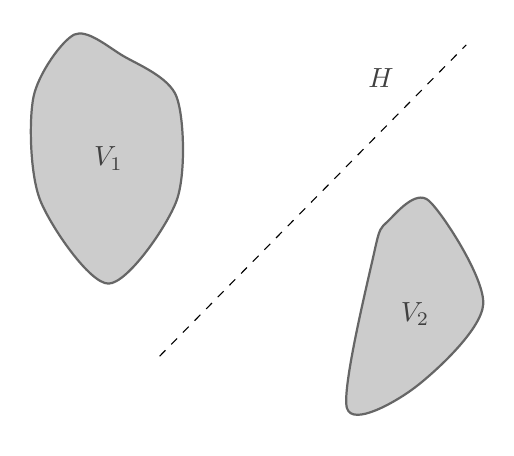
\begin{tikzpicture}
			 \begin{axis}[axis x line=none, axis y line=none]
				\addplot[mark=none, black!60, smooth cycle, thick, fill=gray!40] coordinates {(1,2) (2,1.6) (3,2) (3,2.5) (2.2, 2.7) (1.5, 2.8) (0.9, 2.5)};
				\node[black!75] at (axis cs:2,2.1) [anchor=south] {$V_1$};
				\addplot[dashed] coordinates {(2.75,1.25) (7.25,2.75)};
				\node[black!75] at (axis cs:6,2.5) [anchor=south] {$H$};
				
				\addplot[mark=none, black!60, smooth cycle, thick, fill=gray!40] coordinates {(5.5,1) (6.5,1.1) (7.5,1.5)  (6.7, 2) (6.1, 1.9) (5.9, 1.75)};
				\node[black!75] at (axis cs:6.5,1.35) [anchor=south] {$V_2$};
			 \end{axis}
			\end{tikzpicture}
		\end{figure}
	\[ H = \{ x : x'(x) = \inf_{v_{2} \in V_{2}} x'(v_{2}) \} \]

\begin{satz}[2. Trennungssatz]
	Sei $X$ ein normierter Raum, $V \subset X$ konvex und abgeschlossen. Für $x \notin V$ gibt es ein $x' \in X'$ mit:
		\[ \Re x'(x) < \inf \{ \Re x'(v) : v \in V \} \]	
\end{satz}

\begin{beweis}
	todo, siehe Werner III, Seite 2f % todo, siehe Werner III, Seite 2f 
\end{beweis}



\newpage